\chapter*{Introducción}

Los problemas de iluminacion siempre han sido populares en matematicas. Uno
ejemplo muy conocido, es que la frontera de cualquier conjunto compacto y
convexo $S$ en el plano siempre puede ser iluminado usando tres fuentes de luz
localizadas en el complemento de $S$. Una sencilla prueba de lo anterior puede
obtenerse al encerrar a nuestro conjunto convexo y compacto en un triangulo,
despues colocamos una luz en cada uno de los vertices del triangulo; ver
fig~\ref{im1-1} \\

\begin{figure}[h]
	\centering
	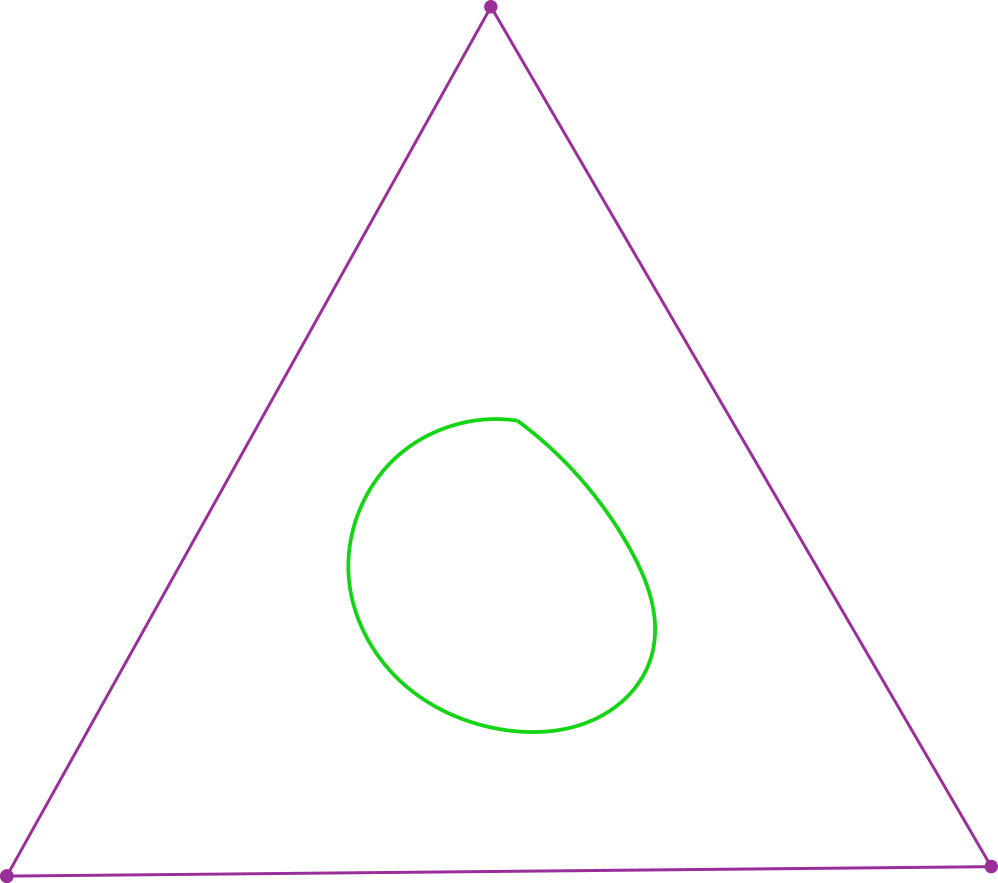
\includegraphics[width=0.5\textwidth]{im1-1}
	\caption{Tres luces iluminan un conjunto convexo y compacto en el Plano.
	\label{im1-1}}
\end{figure}

En 1987, J. O \'Rourke \cite{aguilar_iluminacion_2013}

